% Template for Cogsci submission with R Markdown

% Stuff changed from original Markdown PLOS Template
\documentclass[10pt, letterpaper]{article}

\usepackage{cogsci}
\usepackage{pslatex}
\usepackage{float}
\usepackage{caption}

% amsmath package, useful for mathematical formulas
\usepackage{amsmath}

% amssymb package, useful for mathematical symbols
\usepackage{amssymb}

% hyperref package, useful for hyperlinks
\usepackage{hyperref}

% graphicx package, useful for including eps and pdf graphics
% include graphics with the command \includegraphics
\usepackage{graphicx}

% Sweave(-like)
\usepackage{fancyvrb}
\DefineVerbatimEnvironment{Sinput}{Verbatim}{fontshape=sl}
\DefineVerbatimEnvironment{Soutput}{Verbatim}{}
\DefineVerbatimEnvironment{Scode}{Verbatim}{fontshape=sl}
\newenvironment{Schunk}{}{}
\DefineVerbatimEnvironment{Code}{Verbatim}{}
\DefineVerbatimEnvironment{CodeInput}{Verbatim}{fontshape=sl}
\DefineVerbatimEnvironment{CodeOutput}{Verbatim}{}
\newenvironment{CodeChunk}{}{}

% cite package, to clean up citations in the main text. Do not remove.
\usepackage{apacite}

% KM added 1/4/18 to allow control of blind submission


\usepackage{color}

% Use doublespacing - comment out for single spacing
%\usepackage{setspace}
%\doublespacing


% % Text layout
% \topmargin 0.0cm
% \oddsidemargin 0.5cm
% \evensidemargin 0.5cm
% \textwidth 16cm
% \textheight 21cm

\title{Child language input does not reflect word frequency: Typical and
atypical feature description across development}


\author{{\large \bf Morton Ann Gernsbacher (MAG@Macc.Wisc.Edu)} \\ Department of Psychology, 1202 W. Johnson Street \\ Madison, WI 53706 USA \AND {\large \bf Sharon J.~Derry (SDJ@Macc.Wisc.Edu)} \\ Department of Educational Psychology, 1025 W. Johnson Street \\ Madison, WI 53706 USA}

\begin{document}

\maketitle

\begin{abstract}
Language provides children a powerful source of information about the
world. Blind children learn the same kinds of relationships among visual
categories as sighted children, without any of the relevant visual input
(Landau \& Gleitman, 1985). However, language does not perfectly reflect
the world: the most typical features of natural kinds may often go
unremarked. For instance, adults rarely describe the color of an orange
carrot, as world knowledge makes this description redundant. Given
children's nascent world knowledge, does parents' speech to children
follow this pattern? From longitudinal corpus data of parent-child
communication (Goldin-Meadow et al., 2014) between 14--58 months, we
extracted usage data for 684 high-frequency concrete nouns and
co-occurring adjectives. Independent raters coded the typicality of over
2,000 unique adjective--noun pairs on a 7-point Likert scale. If
language statistics reflect world statistics, description should be
dominated by the typical (strong negative skew); however, across all
ages, we see descriptors concentrated in the atypical range (positive
skewness = 0.65). However, parents were reliably more likely to use
typical descriptors when talking to younger copmared with older
children. Overall, child language input reflects notable more than
typical features, but increased description of typical features early in
development may provide a foothold for young learners.

\textbf{Keywords:}
language input, language acquisition, child-directed speech
\end{abstract}

Children learn a tremendous amount about the structure of the world
around them in just a few short years, from the rules that govern the
movement of physical objects to the hierarchical structure of natural
categories and even relational structures among social and cultural
groups (Baillargeon, 1994; Legare \& Harris, 2016; Rogers \& McClelland,
2004). Where does the information for this rapid acquisition come from?
Undoubtedly, a sizeable component comes from direct experience observing
and interacting with the world (Sloutsky \& Fisher, 2004; Stahl \&
Feigenson, 2015). But another important source of information comes from
the language people use to talk about the world (Landauer \& Dumais,
1997; Rhodes, Leslie, \& Tworek, 2012). For many of the things children
learn about--like the roundness of the earth--the information must come
from language (Harris \& Koenig, 2006). How similar is the information
available from children's direct experience to the information available
in the language children hear?

Two lines of work suggest that they may be surprisingly similar. One
compelling area of work is the comparison of semantic structures learned
by congentinally blind children to those of their sighted peers. In
several domains that would at first blush rely heavily on visual
information, such as color terms or verbs of visual perception (e.g.
\emph{look}, \emph{see}), blind children's semantic similarity judgments
are quite similar to those of sighted children (Landau, Gleitman, \&
Landau, 2009). Further, blind adults' judgments of visual perception
verbs are sensitive to highly detailed information like variation in
intensity (e.g.~blaze vs.~glow), just like sighted adults (Bedny,
Koster-Hale, Elli, Yazzolino, \& Saxe, 2019). A second line of evidence
supporting the similarity of information in perception and language is
the broad success of statistical models trained on language alone in
approximating human judgments across a variety of domains (Devlin,
Chang, Lee, \& Toutanova, 2018; Landauer \& Dumais, 1997; Mikolov,
Sutskever, Chen, Corrado, \& Dean, 2013). Even more compellingly, models
trained on both linguistic usage and perceptual features for some words
can infer the perceptual features of linguistically related words
entirely from the covariation of language and perception (Johns \&
Jones, 2012).

Still, there is reason to believe that some semantic features may be
harder to learn from language than these data suggest. While the
co-occurrence structure of language may provide strong clues that
carrots are like tomatoes, carrots are vegetables, and carrots are eaten
for dinner, they may provide very little evidence that carrots are
orange (Willits, Sussman, \& Amato, 2008). This is because people rarely
use language merely to provide running comentary on the world around
them. Instead, we use language to talk about things we find
interesting--things that are surprising, exciting, or otherwise
divergent from our conversational partners' expectations (Grice, 1975).

Thus, speakers are informative in relation to common knowledge with
their conversational partner and available information in the
environment, not redundant with these other sources of knowledge.
Communication tasks in the lab largely bolster this claim, finding that
people avoid being over- or under-informative when they speak (Mangold
\& Pobel, 1988; MORE CITES) and interpret others' speech as if they are
doing the same (CITES). In particular, speakers are informative in
relation to both the context of objects in the environment and the
typical features of those objects (Mitchell et al., 2013; Westerbeek et
al., 2015; Rubio-Fernandez, 2016). While speakers overwhelmingly refer
to an object that is typical of its category with a bare noun---e.g.,
calling a yellow banana ``a banana''---they often describe more about
the object's features when they are atypical, rarely referring to a
green or blue banana without specifying its color. Listeners are
similarly affected by color description, expecting a color adjective to
be used when an object's color is atypical (Sedivy, 2003).

For things like carrots--that children learn about both from perception
and from language--this issue may be resolved by integrating both
sources of information: Likely almost all of the carrots they see are
orange even if no one comments on them. But for things for which they
lack perceptual access--zoo animals, other social groups, and so on--the
structure of language alone may lead them to have distorted categories.
This may be especially problematic because children's understanding of
the pragmatics of adjective use change significantly over development
(Horowitz \& Frank, 2016).

Should we expect children's categories to be biased in this way, with
typical features underrepresented and atypical features overrepresented?
We examine the typicality of adjectives in a large, diverse corpus of
parent-child ineractions recorded in children's homes to ask whether
parents talking to their children--just like adults speaking and
writing--tend to use adjectives predominantly to mark atypical features.
We find that they do: parents and children overwhelmingly choose to
mention atypical rather than typical features. However, we also find
that parents use adjectives differently over the course of children's
development, noting typical features more often to younger children. We
then ask whether the co-occurrence structure of language nonetheless
captures typicality information, and find that relatively little of it
is represented. Thus, children must either have distorted
representations of categories learned only through language or else
learn typicality through other means.

\textbf{notes for intro word2vec more}

If caregivers use language to mirror the world or to teach their
children about the typical features of things, they should often use
highly typical adjectives to describe nouns. If, on the other hand, they
speak informatively to convey what is atypical or surprising in relation
to their own sophisticated world knowledge, they should more often
mention the atypical features of things.

Information in language goes beyond what can be learned from any one
utterance. Though one might never hear the words /kumquat/ and
/grapefruit/ in the same sentence, their common contexts---other words
like /eat/, /rind/, /tree/, /tart/, and /seeds/---are clues that they
have some similarities. Models of distributional semantics capitalize on
these patterns by representing words using their contexts, and judging
two words to be similar if they are surrounded by similar sets of words.
Though we found that children get more information about atypical than
typical features of objects on the utterance level, perhaps patterns of
language use across many utterances could be used to extract typical
feature information.

\hypertarget{adjective-typicality}{%
\section{Adjective typicality}\label{adjective-typicality}}

In order to determine whether parents use adjectives mostly to mark
atypical features of categories, we analyzed caregiver speech from a
large corpus of parent-child interactions recorded in the home. We
extracted all adjective-noun combinations for concrete nouns, and asked
a sample of Amazon Mechanical Turkers to judge how typical the property
described by each adjective was for the noun it modified. We then
examined both the broad features of this typicality distribution and how
it changed over development.

\hypertarget{corpus}{%
\subsection{Corpus}\label{corpus}}

We used data from the Language Development Project--a large-scale,
longitudinal corpus of parent child-interactions recorded in children's
homes. Families were recruited to be representative of the Chicagoland
area in both socio-economic and racial composition (Goldin-Meadow et
al., 2014). Recordings were taken in the home every 4-months from when
the child was 14-months-old until they were 58-months-old, resulting in
12 timepoints. Each recording was of a 90-minute session in which
parents and children were free to behave as they liked and interact as
much or as little as they liked.

Our sample consistend of all N typically-developing children and their
parents, who were recorded for at least M timepoints. Together, this
resulted in a total of 828,392 distinct parent utterances.
\textbf{SHOULD DO THIS IN CODE}

\hypertarget{stimulus-selection}{%
\subsection{Stimulus Selection}\label{stimulus-selection}}

From these utterances, we extract all of the nouns (using part of speech
tags--\textbf{MANUAL? AUTOMATIC}). Because of our interest in the change
in speech of development, we considered only nouns that appeared at
least once every 3 sessions (i.e.~per developmental year). This yielded
a set of some 2,000 potential target nouns (\textbf{how many did we
lose?}).

We selected from the corpus all N utterances containing any of these
nouns and any word tagged as an adjective. We considered for analysis
all adjective-noun pairs that occurred in any utterance (i.e.~utterances
with one noun and three adjectives were coded as three pairs ). This set
contained a number of high-frequency idiomatic pairs whose typicality
was difficult to classify (e.g., ``good''--``job'';
``little''--``bit''). To resolve this issue, we used human judgments of
words' concreteness to identify and exclude candidate idioms (Brysbaert,
Warriner, \& Kuperman, 2014). We retained for analysis only pairs where
both the adjective and noun were in the top 25\% of the concreteness
ratings. \textbf{GIVE EXAMPLES, SAY HOW MANY}. Finally, all pairs were
given to 7 human coders to judge whether the pair was ``incoherent or
unrelated'' and we thus excluded a further XXX pairs from the sample
(e.g., incoherent pairs such as ``wet'' -- ``brown'', and presumably
errorfully coded pairs such as ``orange'' -- ``orange'').

Thus, our final sample included 2,220 unique adjective-noun pairs drawn
from over 6,000 utterances. The pairs were combinations of 684 distinct
concrete nouns and 118 distinct concrete adjectives. We compiled these
pairs and collected human judgments on Amazon Mechanical Turk for each
pair, as described below. Table \ref{tab:utt_table} contains example
utterances from the final set and typicality judgments from our human
raters.

\begin{table*}[tb]
\centering
\begin{tabular}{llrrrrr}
  \hline
utterance & pair & rating 1 & rating 2 & rating 3 & rating 4 & mean typicality \\ 
  \hline
especially with wooden shoes & wooden-shoe &   2 &   2 &   3 &   2 & 2.75 \\ 
  some of our green bananas too & green-banana &   4 &   3 &   5 &   3 & 3.75 \\ 
  are bananas yellow? & yellow-banana &   5 &   5 &   7 &   6 & 5.75 \\ 
   \hline
\end{tabular}
\caption{Sample typicality ratings from 4 human coders for three adjective-noun pairs drawn from the corpus.} 
\label{tab:utt_table}
\end{table*}

\hypertarget{participants}{%
\subsection{Participants}\label{participants}}

Each participant rated 20 pairs, and each pair was rated by four
participants; we used Dallinger {[}CITE{]}, a tool for automating
complex recruitment on Amazon Mechanical Turk, to balance recruitment.
Overall, we recruited 444 participants to rate 2200 adjective--noun
pairs. After exclusions using an attention check \textbf{what was the
check?}, we retained 8580 judgments, with each adjective--noun pair
retaining at least two judgments.

\hypertarget{design-and-procedure}{%
\subsection{Design and Procedure}\label{design-and-procedure}}

To evaluate the typicality of the adjective--noun pairs that appeared in
parents' speech, we asked participants on Amazon Mechanical Turk to rate
each pair. Participants were presented with a question of the form ``How
common is it for a cow to be a brown cow?'' and asked to provide a
rating on a seven-point scale: (1) never, (2) rarely, (3) sometimes, (4)
about half the time, (5) often, (6) almost always, (7) always.

\begin{CodeChunk}
\begin{figure}[tb]

{\centering 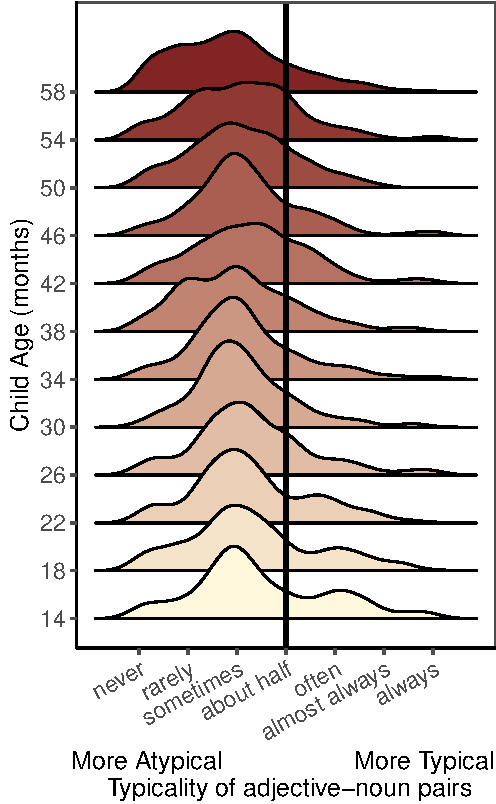
\includegraphics{figs/distribution_plot-1} 

}

\caption[Denisity plots showing the usage amount at each timepoint based on the typicality of the adj-noun pair]{Denisity plots showing the usage amount at each timepoint based on the typicality of the adj-noun pair.}\label{fig:distribution_plot}
\end{figure}
\end{CodeChunk}

\hypertarget{results}{%
\subsection{Results}\label{results}}

If description in child-directed speech mirrors adult-directed speech,
we should see that caregiver description is dominated by modifiers that
are sometimes true of the noun they modify. If instead child-directed
speech privledges redundant or assumed information, caregiver
description should yield a distinct distribution dominated by highly
typical modifiers. As can be seen in Figure \ref{fig:distribution_plot}
parents' description largely focuses on features that are only sometimes
true of the concept.

To confirm this effect statistically, we first centered the ratings
(i.e. ``about half'' was coded 0), and then predicted the rating on each
trial with a mixed effect model with only an intercept and a random
effect of noun
(\texttt{typicality\ \textasciitilde{}\ 1\ +\ (1\textbar{}noun)}). The
intercept was reliably negative, indicating that adjective tends to
refer to atypical features of objects (\(\beta =\) -0.81, \(t =\) -23.4,
\(p\) \textless{} .001). This effect remained significant when each
adjective-noun pair was weighted by it's frequency in the corpus
(\(\beta =\) -0.8, \(t =\) -21.73, \(p\) \textless{} .001). We then
re-estimated these models seperately for each age in the corpus, and
found a reliablly negative intercept for every age group (smallest
effect \(\beta_{14} =\) -0.56, \(t =\) -5.72, \(p\) \textless{} .001).

Examining usage data as a function of typicality (see Figure
\ref{fig:distribution_plot}), we see evidence of a positive skew (0.65).
Data from every time point from 14-58 months seems to show a similar
pattern (skews 0.23 - 0.82). These skews provide further evidence that
the the bulk of caregiver language reflects lower-typicality
adjective-noun pairs.

However, while descriptions at every age tended to point out atypical
features, this effect changed in strength over development. An age
effect added to the previous model was reliably negative, indicating
that parents of older children are relatively more likely to focus on
atypical features (\(\beta =\) -0.06, \(t =\) -2.09, \(p =\) .036). This
effect also remained significant when pairs were weighted according the
their frequency (\(\beta =\) -0.14, \(t =\) -4.76, \(p\) \textless{}
.001).

\hypertarget{adult-to-adult-speech.}{%
\subsubsection{Adult to adult Speech.}\label{adult-to-adult-speech.}}

Next, we briefly confirm that adult to adult speech shows the similar
usage pattern using an identical analysis framework on usage data from
the Corpus of Contemporary American English (COCA). Using the set of
adjective-noun pairs for which we have judgments from our analysis of
caregiver speech, we repeat our analysis of usage frequencies for a set
of 1,357 distinct adjective-noun pairs.

As predicted, an identical mixed effects model predicting typicality
from usage shows that adult-directed speech speech is significantly
biased toward description of atypical features (\emph{B} XXX, \emph{p}
\textless{} YYY ). ADS also shows a similar a positive skew (0.68), such
that the bulk of language reflects adjective-noun pairs rated
\textless{} 4 on typicality (i.e. `sometimes', `rarely' or `never').

The usage distributions in adult-directed speech seem qualitatively
similar to the distributions we found in child-directed speech. In sum,
these data suggest that even when talking with very young children,
caregiver speech structures information similarly to adult-directed
speech.

The difference of settings makes it difficult to compare these data
directly with our data from the Language Development Project corpus.
Four of the COCA datasets are drawn from written texts, which puts in
place distinct language pressures and removes visual common ground.
While there is one subset of the corpus drawn from spoken data, those
utterances come from TV and radio programs. All of these settings are
likely quite different environements for language than the naturalistic
in-home setting that our Language Development Project corpus draws from.
In light of these differences, any observed similarity in usage seems
remarkable.

\hypertarget{child-speech.}{%
\subsubsection{Child Speech.}\label{child-speech.}}

What kind of information is contained in children's own speech? By
analyzing children's own utterances, we can determine when children come
to use description in a way that looks like caregiver speech. Are
children mirroring adult-like uses of description even from a young age,
or are they choosing to describe more typical features of the world?

The Language Development Corpus contains 442,048 child utterances. Using
the set of adjective-noun pairs for which we have judgments from our
analysis of caregiver speech, we repeat our analysis on usage data for a
set of 533 distinct adjective-noun pairs.

While preliminary, an identical mixed effects model predicting
typicality from usage shows that children's speech is signficantly
biased toward description of atypical features (\emph{B} XXX, \emph{p}
\textless{} YYY ). Mirroring caregiver and adult-adult speech,
children's productions show a positive skew (0.61, comapre with skewness
= 0.65 seen in the adults), such that the bulk of language reflects
adjective-noun pairs rated \textless{} 4 on typicality (i.e.
`sometimes', `rarely' or `never').

\hypertarget{talk-about-the-highly-typical.}{%
\subsubsection{Talk about the
Highly-Typical.}\label{talk-about-the-highly-typical.}}

Though there is striking consistency of description in caregiver speech
across development, we found parents of older children were more likely
to refer to atypical features. In line with our hypotheses, it seems
that caregivers are more likely to provide description of typical
features for their young children, compared with older children. To
confirm this intuition, we defined adjectives as highly-typical if
Turkers judged them to be `often', `almost always', or `always' true. We
predicted whether each judgment was highly typical from a mixed-effects
logistic regression with a fixed effect of age (log-scaled) and a random
effect of noun. Age was a highly-reliable predictor (\(\beta =\) -0.97,
\(t =\) -6.11, \(p\) \textless{} .001). While children at all ages hear
more talk about what is atypically true (Figure
\ref{fig:distribution_plot}), younger children hear relatively more talk
about what is typically true than older children do (Figure
\ref{fig:prototypical_plot}).

\begin{CodeChunk}
\begin{figure}[tb]

{\centering 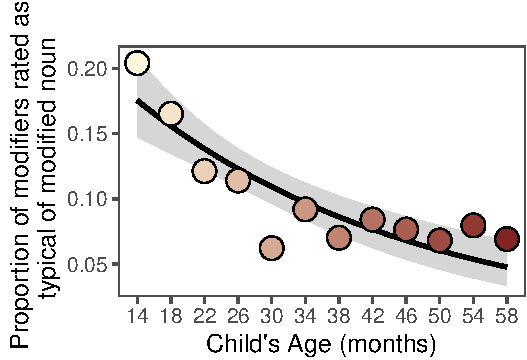
\includegraphics{figs/prototypical_plot-1} 

}

\caption[Proportion of caregiver description that is about typically-true features, as a function of age]{Proportion of caregiver description that is about typically-true features, as a function of age.}\label{fig:prototypical_plot}
\end{figure}
\end{CodeChunk}

\hypertarget{discussion}{%
\subsection{Discussion}\label{discussion}}

In sum, language is used to discuss atypical, rather than typical,
features of the world. Description in caregiver speech largely mirrors
the usage patterns that we observed in adult-adult speech, suggesting
that these patterns arise from general communication pressures. Indeed,
even children's own productions show a similar usage pattern, with more
description of atypical features of the world as early as we can
measure.

It should be noted that children's utterances come from naturalistic
conversations with caregivers, and their pattern of description is
likely highly dependent on that caregiver's utterances. That is, if a
parent chooses to describe the \emph{purpleness} of a cat in book, the
child may well respond by asking about that same feature. Thus, some of
the children's use of atypical description may be prompted by a
parent-led discourse. Future analyses would need to better disentangle
the extent to which children's productions are imitative of caregivers.

While children's own descriptions largely mirror adults', the
descriptions children hear change over, becoming increasingly focused on
atypical features. The higher prevalance of typical descriptors in early
development may help young learners; however, even at the earliest point
we measured, the bulk of language input describes atypical features.

Across adult, parent, and child language corpora, we find robust
evidence that language use systematically overerpresents atypical
features. This usage aligns with the idea that language is used
informatively in relation to background knowledge about the world. It
may pose a problem, however, for young language learners with
still-developing world knowledge. If language does not transparently
convey the typical features of objects, and instead (perhaps
misleadingly) notes the atypical ones, how might children come to learn
what objects are typically like? One possibility is that information
about typical features is captured in regularities across many
utterances. If this is true, language may still be an important source
of information about typicality as children may be able to extract more
accurate typicality information by tracking second-order co-occurence.

\hypertarget{other-ways-of-extracting-structure-from-language}{%
\section{Other Ways of Extracting Structure from
Language}\label{other-ways-of-extracting-structure-from-language}}

Much information can be gleaned from language that does not seem
available at first glance. From language alone, simple distributional
learning models can recover enough information to perform comparably to
non-native college applicants on the Test of English as a Foreign
Language (Landauer \& Dumais, 1997). Recently, Lewis, Zettersten, \&
Lupyan (2019) demonstrated that even nuanced feature information may be
learnable through distributional semantics alone, without any complex
inferential machinery. We take a similar approach to ask whether a
distributional semantics model trained on the language children hear can
capture typical feature information.

\hypertarget{word2vec}{%
\subsubsection{Word2Vec}\label{word2vec}}

To test this possibility, we trained word2vec, a model that predicts
words using their contexts, on the same corpus of child-directed speech
used in our first set of analyses. Our model is a
continuous-bag-of-words word2vec model trained using the package gensim
(Řehůřek \& Sojka, 2010). If the model captures information about the
typical features of objects, we should see that the model's word pair
similarities are correlated with the typicality ratings we elicited from
human raters.

\hypertarget{results-1}{%
\subsubsection{Results}\label{results-1}}

We find that similarities in the model have near zero correlation with
human adjective--noun typicality ratings (r = 0.018). This is in spite
of better correlations with large sets of human similarity judgments
between different kinds of word pairs (correlation with wordsim353,
0.37; correlation with simlex, 0.15). This suggests that statistical
patterns in child-directed speech are likely insufficient to encode
information about the typical features of objects, despite encoding at
least some information about word meaning more broadly. However, the
corpus on which we trained this model was small; perhaps our model did
not get enough language to draw out the patterns that would reflect the
typical features of objects. To test this possibility, we asked whether
word vectors trained on a much larger corpus---English
Wikipedia---strongly correlate with typicality ratings. We find that
while the correlation between similarities in the Wikipedia--trained
model and human noun--adjective typicality ratings is stronger, it is
still fairly weak at r = 0.24. Strikingly, the correlation between
similarities in our model and similarities in the Wikipedia-trained
models is stronger (r = 0.33) than either model's correlations with
human judgments. This suggests that these models are picking up on some
systematic associations between nouns and adjectives, but not typical
ones. Overall, these results suggest that models of distributional
semantics fail to extract typical feature information from language in
which atypical features are more often described.

\begin{CodeChunk}
\begin{figure}[tb]

{\centering 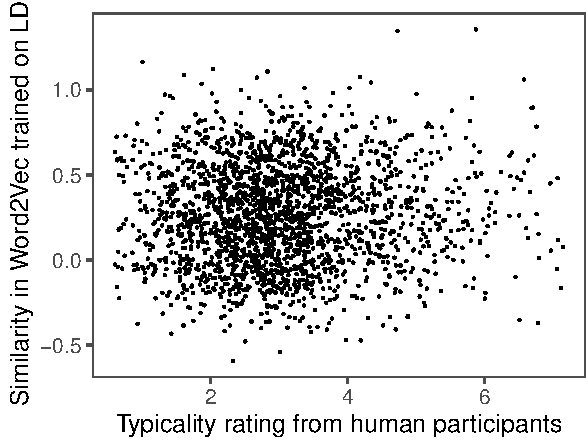
\includegraphics{figs/word2vec1-1} 

}

\caption[Correlation between vector similarities in word2vec (trained on the LDP corpus) and human-rated typicality judgments for our noun-adjective pairs]{Correlation between vector similarities in word2vec (trained on the LDP corpus) and human-rated typicality judgments for our noun-adjective pairs.}\label{fig:word2vec1}
\end{figure}
\end{CodeChunk}

\begin{CodeChunk}
\begin{figure}[tb]

{\centering 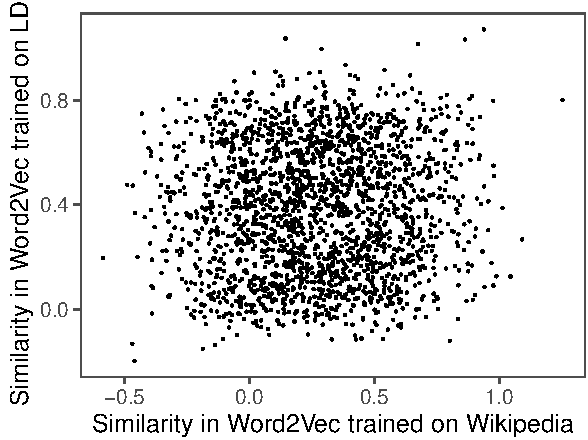
\includegraphics{figs/word2vec2-1} 

}

\caption[Correlation between vector similarities in word2vec trained on the LDP corpus and vector similarities in word2vec trained on English Wikipedia for our noun-adjective pairs]{Correlation between vector similarities in word2vec trained on the LDP corpus and vector similarities in word2vec trained on English Wikipedia for our noun-adjective pairs.}\label{fig:word2vec2}
\end{figure}
\end{CodeChunk}

\hypertarget{general-discussion}{%
\section{General Discussion}\label{general-discussion}}

Language provides children a rich source of information about the world.
However, this information is not always transparently available:
language's use to comment on the atypical and surprising means it does
not perfectly mirror the world. Among adult conversational partners
whose world knowledge is well-aligned, this characteristic of language
allows people to converse informatively and not redundantly. But between
a child and caregiver whose world knowledge is asymmetric, this pressure
competes with other demands: what is minimally informative to an adult
may be misleading to a child. In this work, we demonstrate that this
pressure structures language to create a peculiar learning environment:
one in which caregivers predominantly point out the atypical features of
things.

How, then, do children learn about the typical features of things from
such an environment? While younger children may gain an importnat
foothold from hearing more description of typical features, they still
face language dominated by atypical description. Further when we looked
at more nuanced ways\ldots{} , we found that models of distributional
semantics capture little typical feature information.

Of course, one source of information that may simplify this problem is
perceptual information from the world itself. In many cases, perceptual
information may swamp information from language; children likely see
enough orange carrots in the world to outweigh hearing ``purple
carrot.'' It remains unclear, however, how children learn about
categories for which they have scarcer evidence. Indeed, language
information likely swamps perceptual information for many other
categories, such as abstract concepts or those that cannot be learned
about by direct experience. Given that the present work is limited to
concrete concepts, we can only speculate about the information
caregivers provide about abstract concepts. But, if abstract concepts
pattern similarly to concrete objects, children are in a particularly
difficult bind. Though perceptual information is undoubtedly useful in
learning about the typical features of things, it remains to be
explained how children learn what is typical when this perceptual
information is scant, irrelevant, or incomplete.

Another possibility is that children expect language to be used
informatively at a young age. Under this hypothesis, their language
environment is not misleading at all. If young children expect
adjectives to mark atypical features, they can use description and the
lack thereof to learn more about the world around them. Lab studies find
that children expect interlocutors to be informative in relation to
their prior knowledge by the age of 2 (Akhtar et al., 1996) and that
5--6-year-old children are roughly informative with respect to their
interlocutor's perspective in a referential communication task (Nadig \&
Sedivy, 2002). More naturalistic studies find that children at the
one-word stage selectively imitate words that convey new
information---that is, words that are informative with respect to what
is obvious or assumed in the environment---when describing events
(Greenfield \& Zukow, 1978). The idea that young children understand the
informative purpose of language is consistent with our finding that even
young children also largely choose to describe atypical features. Though
this effect can be explained by simpler means such as salience or
mimicry, it suggests that caregivers and children may be usefully
aligned in the aspects of the world they choose to talk about.

Whether adult-directed, child-directed, or a child's own speech,
language is used with remarkable consistency: people talk about the
atypical. Though parents might reasonably be broadly over-informative in
order to teach their children about the world, this is not the case.
This presents a potential puzzle for young learners who have limited
world knowledge and limited pragmatic inferential abilities. Perceptual
information and nascent pragmatic abilities may help fill in the gaps,
but much remains to be explored to link these explanations to actual
learning. Communication pressures are pervasive forces structuring the
language children hear, and future work must disentangle whether
children capitalize on them or are misled by them in learning about the
world.

\hypertarget{acknowledgements}{%
\section{Acknowledgements}\label{acknowledgements}}

Place acknowledgments (including funding information) in a section at
the end of the paper.

\hypertarget{references}{%
\section{References}\label{references}}

\setlength{\parindent}{-0.1in} 
\setlength{\leftskip}{0.125in}

\noindent

\hypertarget{refs}{}
\leavevmode\hypertarget{ref-baillargeon1994}{}%
Baillargeon, R. (1994). How do infants learn about the physical world?
\emph{Current Directions in Psychological Science}, \emph{3}(5),
133--140.

\leavevmode\hypertarget{ref-bedny2019}{}%
Bedny, M., Koster-Hale, J., Elli, G., Yazzolino, L., \& Saxe, R. (2019).
There's more to ``sparkle'' than meets the eye: Knowledge of vision and
light verbs among congenitally blind and sighted individuals.
\emph{Cognition}, \emph{189}, 105--115.

\leavevmode\hypertarget{ref-brysbaert2014}{}%
Brysbaert, M., Warriner, A. B., \& Kuperman, V. (2014). Concreteness
ratings for 40 thousand generally known english word lemmas.
\emph{Behavior Research Methods}, \emph{46}(3), 904--911.

\leavevmode\hypertarget{ref-devlin2018}{}%
Devlin, J., Chang, M.-W., Lee, K., \& Toutanova, K. (2018). Bert:
Pre-training of deep bidirectional transformers for language
understanding. \emph{arXiv Preprint arXiv:1810.04805}.

\leavevmode\hypertarget{ref-grice1975}{}%
Grice, H. P. (1975). Logic and conversation. In \emph{Speech acts} (pp.
41--58). Brill.

\leavevmode\hypertarget{ref-harris2006}{}%
Harris, P. L., \& Koenig, M. A. (2006). Trust in testimony: How children
learn about science and religion. \emph{Child Development},
\emph{77}(3), 505--524.

\leavevmode\hypertarget{ref-horowitz2016}{}%
Horowitz, A. C., \& Frank, M. C. (2016). Children's pragmatic inferences
as a route for learning about the world. \emph{Child Development},
\emph{87}(3), 807--819.

\leavevmode\hypertarget{ref-johns2012}{}%
Johns, B. T., \& Jones, M. N. (2012). Perceptual inference through
global lexical similarity. \emph{Topics in Cognitive Science},
\emph{4}(1), 103--120.

\leavevmode\hypertarget{ref-landau2009}{}%
Landau, B., Gleitman, L. R., \& Landau, B. (2009). \emph{Language and
experience: Evidence from the blind child} (Vol. 8). Harvard University
Press.

\leavevmode\hypertarget{ref-landauer1997}{}%
Landauer, T. K., \& Dumais, S. T. (1997). A solution to plato's problem:
The latent semantic analysis theory of acquisition, induction, and
representation of knowledge. \emph{Psychological Review}, \emph{104}(2),
211.

\leavevmode\hypertarget{ref-legare2016}{}%
Legare, C. H., \& Harris, P. L. (2016). The ontogeny of cultural
learning. \emph{Child Development}, \emph{87}(3), 633--642.

\leavevmode\hypertarget{ref-lewis2019}{}%
Lewis, M., Zettersten, M., \& Lupyan, G. (2019). Distributional
semantics as a source of visual knowledge. \emph{Proceedings of the
National Academy of Sciences}, \emph{116}(39), 19237--19238.

\leavevmode\hypertarget{ref-mikolov2013}{}%
Mikolov, T., Sutskever, I., Chen, K., Corrado, G. S., \& Dean, J.
(2013). Distributed representations of words and phrases and their
compositionality. In \emph{Advances in neural information processing
systems} (pp. 3111--3119).

\leavevmode\hypertarget{ref-rhodes2012}{}%
Rhodes, M., Leslie, S.-J., \& Tworek, C. M. (2012). Cultural
transmission of social essentialism. \emph{Proceedings of the National
Academy of Sciences}, \emph{109}(34), 13526--13531.

\leavevmode\hypertarget{ref-rogers2004}{}%
Rogers, T. T., \& McClelland, J. L. (2004). \emph{Semantic cognition: A
parallel distributed processing approach}. MIT press.

\leavevmode\hypertarget{ref-rehurek2010}{}%
Řehůřek, R., \& Sojka, P. (2010). Software Framework for Topic Modelling
with Large Corpora. In \emph{Proceedings of the LREC 2010 Workshop on
New Challenges for NLP Frameworks} (pp. 45--50). Valletta, Malta: ELRA.

\leavevmode\hypertarget{ref-sedivy2003}{}%
Sedivy, J. C. (2003). Pragmatic versus form-based accounts of
referential contrast: Evidence for effects of informativity
expectations. \emph{Journal of Psycholinguistic Research}, \emph{32}(1),
3--23.

\leavevmode\hypertarget{ref-sloutsky2004}{}%
Sloutsky, V. M., \& Fisher, A. V. (2004). Induction and categorization
in young children: A similarity-based model. \emph{Journal of
Experimental Psychology: General}, \emph{133}(2), 166.

\leavevmode\hypertarget{ref-stahl2015}{}%
Stahl, A. E., \& Feigenson, L. (2015). Observing the unexpected enhances
infants' learning and exploration. \emph{Science}, \emph{348}(6230),
91--94.

\leavevmode\hypertarget{ref-willits2008}{}%
Willits, J. A., Sussman, R. S., \& Amato, M. S. (2008). Event knowledge
vs. Verb knowledge. In \emph{Proceedings of the 30th annual conference
of the cognitive science society} (pp. 2227--2232).

\bibliographystyle{apacite}


\end{document}
